\newpage 
% %%%%%%%%%%%%%%%%%%%%%%%%%%%%%%%%%%%%%%%%%%%%%%%%%%%
\section{The BDI Learning Framework}\label{sec:framework}
% %%%%%%%%%%%%%%%%%%%%%%%%%%%%%%%%%%%%%%%%%%%%%%%%%%%

We begin by briefly reviewing the basic agent programming framework that will be used throughout the paper~\cite{airiau09:enhancing,singh10:extending,singh10:learning}, which is a seamless integration of standard Belief-Desire-Intention (BDI) agent-oriented programming~\cite{Rao96:AgentSpeak,WooldridgeBook} with decision tree learning~\cite{Mitchell97:ML}. 

Generally speaking, BDI agent-oriented programming languages are built around an explicit representation of propositional attitudes (e.g., beliefs, desires, intentions, etc.). A BDI architecture addresses how these components are represented, updated, and processed to determine the agent's actions.
%%
There are a plethora of agent programming languages and development platforms in the BDI tradition, including
%such as \PRS\ \cite{Georgeff89-PRS},
\JACK~\cite{BusettaRHL:AL99-JACK}, 
\JADEX~\cite{Pokahr:EXP03-JADEX}, and
%\TAPL~\cite{Hindriks99:Agent} and
%\DAPL~\cite{Dastani:JAAMAS08-2APL}, 
\JASON~\cite{jasonbook}
%, and SRI's \SPARK~\cite{MorelyM:AAMAS04-SPARK}, 
among others. 
%%
Specifically, a BDI intelligent agent systematically chooses and executes \emph{plans} (i.e., operational procedures) to achieve or realize its goals, called \emph{events}.
%%
Such plans are extracted from the so-called agent's \emph{plan library}, which encode the ``know-how'' information of the domain the agent operates on.
%%
For instance, the plan library of an unmanned air vehicle (UAV) agent controller may include several plans to address the event-goal of landing the aircraft. Each plan is associated with a \emph{context condition} stating under which belief conditions the plan is a sensible strategy for resolving the goal in question. Whereas some plans for landing the aircraft may only be suitable under normal weather conditions, other plans may only be used under emergency operations.
%%%
Besides the actual execution of domain actions (e.g., lifting the flaps), a plan may require the resolution of (intermediate) sub-goal events (e.g., obtain landing permission from air control tower). As a result, the execution of a BDI system can be seen as a \textit{context sensitive subgoal expansion}, allowing agents to ``act as they go'' by making \emph{plan choices} at each level of abstraction with respect to the current situation. The use of plans' context (pre)conditions to make choices as late as possible, together with the built-in goal-failure mechanisms, ensures that the system is responsive to changes in the environment. 




It is not hard to see that, by grouping together plans responding to the same event type, the agent's plan library can be seen as
a set of goal-plan tree templates (e.g., Figure~\ref{fig:confidence}): a goal-event node (e.g., goal $G_1$) has children representing the alternative \emph{relevant} plans for achieving it (e.g., $P_a,P_b$ and $P_c$); and a plan node (e.g., $P_f$), in turn, has children nodes representing the subgoals (including primitive actions) of the plan (e.g., $G_4$ and $G_5$). These structures, can be seen as AND/OR trees: for a plan to succeed all the subgoals and actions of the plan must be successful (AND); for a subgoal to succeed one of the plans to achieve it must succeed (OR). Leaf plans are meant to directly interact with the environment and so, in a given world state, they can either succeed or fail when executed; this is marked accordingly in the figure for some particular world (of course such plans may behave differently in other states).


As can be seen, adequate plan selection is critically important in BDI systems. Whereas standard BDI platforms leverage domain expertise by means of the \emph{fixed} logical context conditions of plans, in this work, we are interested in exploring how a situated agent may \emph{learn} or \emph{improve} its plan selection mechanism based on experience, in order to better realize its goals.
%%
To that end, it was proposed to generalize the account for plans' context conditions to decision trees~\cite{Mitchell97:ML} that can be learnt over time~\cite{airiau09:enhancing,singh10:extending,singh10:learning}. The idea is simple: \emph{the decision tree of an agent plan provides a judgement as to whether the plan is likely to succeed or fail for the given situation.}
%%
By suitably \emph{learning} the structure of such decision tree and adequately \emph{using} such decision trees, we expect the agent to be able to improve its performance over time and release the domain modeller to encode ``perfect'' plan preconditions. Note that the classical boolean context conditions provided by the designer could (and generally will) still be used as initial necessary but possibly insufficient requirements for each plan that will be further \emph{refined} over time in the course of trying plans in various world states.


Under the new BDI learning framework, two mechanisms become crucial. First, of course, a principled approach to learning such decision trees based on execution experiences is needed. Second, an adequate plan selection scheme compatible with the new type of plans' preconditions is required.
%%
To select plans based on information in the decision trees, the work reported in \cite{singh10:extending,singh10:learning} used a probabilistic method that chooses a plan based on its believed likelihood of success in the given situation. This approach provides a balance between exploitation (we choose plans with relatively higher success expectations more often), and exploration (we sometimes choose plans with lower success expectation to get better confidence in their believed applicability by trying them in more situations). This balance is important because ongoing learning influences future plan selection, and subsequently whether a good solution is learnt.


\begin{figure}[t]
\begin{center}
%\resizebox{.45\textwidth}{!}{
%!TEX root = ../ijcai11storage.tex
\begin{tikzpicture}[level distance=1.0cm]
\tikzstyle{succ}=[label=below:$\surd$]
\tikzstyle{fail}=[label=below:$\times$]
\tikzstyle{trace}=[solid,style=circle,fill=black!20,above left=0.15cm,scale=.7]

\tikzstyle{planbox}=[draw,minimum height=0.6cm,minimum width=0.65cm]
\tikzstyle{goalbox}=[draw,minimum height=0.6cm,minimum width=0.65cm,rounded corners=0.2cm]
\tikzstyle{planbox2}=[planbox,pattern=north west lines,pattern color=black!30]
\tikzstyle{goalbox2}=[goalbox,pattern=north west lines,pattern color=black!30]
\tikzstyle{goalbox3}=[goalbox,fill=black!20]
\tikzstyle{planbox3}=[planbox,fill=black!20]

	
\tikzstyle{level 1}=[sibling distance=2.7cm] 
\tikzstyle{level 2}=[sibling distance=0.9cm] 
\tikzstyle{level 3}=[sibling distance=2.7cm]
\tikzstyle{level 4}=[sibling distance=0.9cm]

\node[planbox3,solid] {$P$}
		child {node[goalbox2] {$G_{1}$}
			child {node[planbox2] {$P_{a}$}
				child {node[goalbox2] {$G_{3}$}
					child {node[planbox,fail] {$P_{g}$}}
					child {node[planbox,fail] {$P_{h}$}}
					child {node[planbox2,succ] {$P_{i}$}}
				}
			}
			child {node[planbox,fail] {$P_{b}$}}
			child {node[planbox,fail] {$P_{c}$}}
		}
		child {node[goalbox3] {$G_{2}$}
			child {node[planbox,fail] {$P_{d}$}}
			child {node[planbox,fail] {$P_{e}$}}
			child {node[planbox3] {$P_f$}
				child {node[goalbox2] {$G_{4}$}
					child {node[planbox,fail] {$P_{j}$}}
					child {node[planbox2,succ] {$P_{k}$}}
					child {node[planbox,fail] {$P_{l}$}}
				}
				child {node[goalbox3] {$G_{5}$}
					child {node[planbox3,succ] {$P_{m}$}}
					child {node[planbox,fail] {$P_{n}$}}
					child {node[planbox,fail] {$P_{o}$}}
				}
			}
		}
		
;

\end{tikzpicture}

%}
\end{center}
\caption{An example goal-plan hierarchy.}
\label{fig:confidence}
\end{figure}

When it comes to the learning process, the training set for a given plan's decision tree contains samples of the form $[w, o]$, where $w$ is the world state---a vector of discrete attributes---in which the plan was executed and $o$ is the execution outcome, namely, success or failure. Initially, the training set is empty and grows as the agent tries the plan in various world states and records each execution result. 
%%
Since the decision tree inductive bias is a preference for smaller trees, one expects that the decision tree learnt to be built from only those world attributes that are relevant to the corresponding plan's (real) context condition.
%%
Now, due to the hierarchical nature of the plan-goal hierarchy being executed by the agent (c.f. Figure~\ref{fig:confidence}), it is possible that the failure of a plan (e.g., $P$) is only due to a poor plan selection lower in the hierarchy (e.g., $P_l$ is selected for goal $G_4$).
%%
To deal with this issue, the work in \cite{airiau09:enhancing} uses a plan ``stability" measure to take failures into account only when the agent is sufficiently sure that the failure was not due to poor sub-plan choices. Another approach reported is to adjust the plan selection probability based on some measure of our ``confidence'' in the decision tree~\cite{singh10:learning} which considers the reliability of a plan's decision tree to be proportional to the number of sub-plan choices (or paths below the plan in the goal-plan hierarchy) that have been explored already: the greater the coverage, the more we have explored and the greater the confidence in the resulting decision tree. 

\paragraph{An energy storage domain example}

% Energy storage enables increasing levels of renewable energy in our electricity system, and the rapidly maturing supply chains for several battery technologies encourages electricity utilities, generators, and customers to consider using large battery systems. 



\newcommand{\pSet}{\mathname{Set*}}
\newcommand{\pSetCharge}{\mathname{SetCharge}}
\newcommand{\pSetDischarge}{\mathname{SetDischarge}}
\newcommand{\pSetNotUsed}{\mathname{SetNotUsed}}
\newcommand{\pExecute}{\mathname{Execute}}

\newcommand{\cSatisfies}{\psi}

\newcommand{\aSet}{\mathname{set}}
\newcommand{\aOperate}{\mathname{operate}}
\newcommand{\aEvaluate}{\mathname{evaluate}}

\begin{figure*}[t]
\begin{center}
\subfigure[Use case scenario for a modular battery system.]{\label{fig:usecase}
\resizebox{.9\columnwidth}{!}{%!TEX root = ../aamas11storage.tex
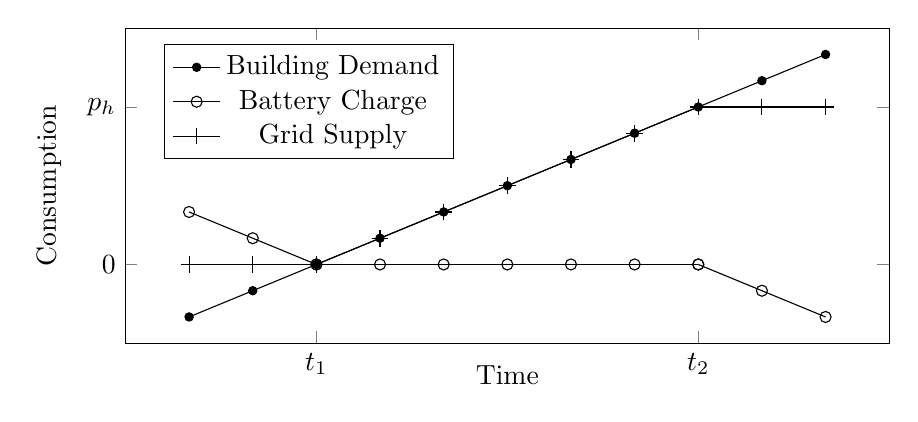
\begin{tikzpicture}

\begin{axis}[
width=0.8\columnwidth,height=4cm,scale only axis,
axis line style={-}, xtick style={-}, ytick style={-},
xlabel=Time,
ylabel=Consumption,
every axis y label/.style={at={(-0.1,0.5)},rotate=90,anchor=center}, 
every axis x label/.style={at={(0.5,-0.1)},anchor=center}, 
%grid=both, grid style={style=densely dotted},
xtick={2,8},
xticklabels={$t_1$,$t_2$},
ytick={0,6},
yticklabels={$0$,$p_h$},
legend style={at={(0.05,0.95)},anchor=north west}
] 

% Draw the Demand-Supply curve
\addplot[-,mark=*,mark size=1.5] expression[domain=0:10,samples=11] {x-2};
\addlegendentry{Building Demand} 

% Draw the Battery curve
\addplot[-,mark=o,mark size=2] expression[forget plot,domain=0:2,samples=3] {2-x}; 
\addplot[-,mark=o,mark size=2] expression[forget plot,domain=2:8,samples=7] {0}; 
\addplot[-,mark=o,mark size=2] expression[domain=8:10,samples=3] {8-x}; 
\addlegendentry{Battery Charge} 

% Draw the Grid supply curve
\addplot[-,mark=+,mark size=3] expression[forget plot,domain=0:2,samples=3] {0}; 
\addplot[-,mark=+,mark size=3] expression[forget plot,domain=2:8,samples=7] {x-2}; 
\addplot[-,mark=+,mark size=3] expression[domain=8:10,samples=3] {6}; 
\addlegendentry{Grid Supply} 
\end{axis} 
\end{tikzpicture} 
}
}
\qquad
\subfigure[Goal-plan hierarchy for a $k$-modules battery system.]{\label{fig:gptree}
\resizebox{.9\columnwidth}{!}{%!TEX root = ../aamas11storage.tex
\begin{tikzpicture} [level distance=8.0em]
\tikzstyle{planbox}=[draw,text width=11.0em,rectangle split,rectangle split parts=3]
\tikzstyle{goalbox}=[draw,rounded corners=1.25em,minimum height=3em,minimum width=5em]

	
\tikzstyle{level 1}=[sibling distance=13.0em] 
\tikzstyle{level 2}=[level distance=7.0em] 

\node[goalbox,solid] {$G($r,k,s$)$}
	child {node[planbox] {$SetCharge$ 
			\nodepart{second} $\psi:satisfies(r,k,s,C),$\\$k>0$
			\nodepart{third} $set(k,C)$
		}
		child {node[goalbox] {$G($r,k-1,s'$)$}}
	}
	child {node[planbox] {$SetDischarge$ \nodepart{second}
			\nodepart{second} $\psi:satisfies(r,k,s,D),$\\$k>0$
			\nodepart{third} $set(k,D)$
		}
		child {node[goalbox] {$G($r,k-1,s'$)$}}
	}
	child {node[planbox] {$SetNotUsed$ \nodepart{second}
			\nodepart{second} $\psi:satisfies(r,k,s,N),$\\$k>0$
			\nodepart{third} $set(k,N)$
		}
		child {node[goalbox] {$G($r,k-1,s'$)$}}
	}
	child {node[planbox] {$Execute$ 
			\nodepart{second} $\psi:k==0$
			\nodepart{third} $operate()$ \\$evaluate()$
		}
	}
;

\end{tikzpicture}


}
}
\caption{An energy storage scenario.}
\end{center}
\label{fig:energystorage}
\end{figure*}

Consider a smart office building comprising of a set of loads (e.g., appliances in the building), some renewable sources (e.g., solar panels on the roof and a local wind turbine), and a \emph{modular battery system}. The building is connected to the main grid, and economics govern that the overall grid power demand of the building be maintained within the range $[0:p_h]$; see Figure~\ref{fig:usecase}. 
%%
Since there is little control over the demand in the building, and certainly no control over the renewable generation, it is possible that the building power consumption falls outside this range for some period in the day. For instance, if the renewable generation is high relative to the building loads, then net consumption may fall below $0$ (e.g., period prior to $t_1$); whereas if demand is higher than generation, then the net building consumption may rise above $p_h$ (e.g., period after $t_2$). 

While net demand is fixed for all practical purposes, we do have control over the use of the battery system (Battery Charge). Hence, by suitably ordering the battery system to charge (i.e., act as a load) or discharge (i.e., act as a generator) at determined rates, it is possible to influence the building net demand. 
% Figure \ref{fig:usecase} shows how the appropriate battery response (Battery Charge) added to the net building consumption (Building Demand) ensures that the power drawn from the grid (Grid Supply) is maintained within the desired range.
%%
Large battery systems usually comprise of multiple modules that can be controlled independently.  Modules may be operated in synchrony, but there are often strategic reasons for keeping some modules in different states.  For example, if it is undesirable to change the direction of power flow between charging and discharging too frequently, a subset of modules may be used for each direction until it is necessary to swap their roles. Also, some technologies have specific requirements, such as zinc-bromine flow batteries needing complete discharges at regular intervals to ``strip'' the zinc plating and hence ensuring irregularities never accumulate. Where they exist, such requirements place further constraints on module control.

So, given a large battery installation, we are interested in a mechanism to achieve certain desired rate of charging or discharging, by suitably setting each module in the battery---the overall rate is the sum over the modules' rates.  
%%
For simplicity, we assume homogeneous capacity $c$ of the modules (but with possibly different chemical properties and constraints), and hence an overall system capacity of $c*n$ (where $n$ is the total number of modules in the system). Each module, in turn, may be configured as charging ($+c$), discharging ($-c$), or not in use ($0$). By appropriately setting each module's operational state, the total response of the battery system may be adjusted in steps of $\pm c$.
%%
While hardwired control is indeed possible, it is not ideal due to the fact that battery performance is susceptible to changes over time---modules tend to lose actual capacity---and may diverge from normal. 
%%
What is required is an \emph{adaptable} control mechanism that accounts for such drift. 
%%
Figure~\ref{fig:gptree} depicts a BDI controller for this application. Top-level goal-even $G(r,k,s)$ is meant to request a battery charge/discharge (normalized) rate of $r \in [-1.0:+1.0]$, where $-1.0$ ($1.0$) indicates maximum discharge (charge) rate, $s$ stands for the current state of the battery system as per sensor readings, and $k$ is (initially) the number of modules in the system. 
%%
The BDI controller works by recursively \emph{configuring} each module for the period in question using the plans $\pSetCharge$ (\emph{charging} at rate $+c$), $\pSetDischarge$ (\emph{discharging} at rate $cc$), and $\pSetNotUsed$ plans (disconnect module), and, finally, after all modules have been configured, physically operating the battery for the period using the $\pExecute$ plan. 
% At any point in the execution of the controller, then, the {\em active execution trace} always consists of the selection of $k$ high level $Set*$ plans followed by the selection of the $Execute$ leaf plan. 
%%
% Plan $\pSetCharge$ sets the $k$-th module to {\em charging} (state $+c$) for the period in question; similarly, plan $\pSetDischarge$ sets the $k$-th module to {\em discharging} (state $-c$) for the period.  Plan $\pSetNotUsed$, on the other hand, set the module to a neutral not-in-use state (state $0$). Finally, when all modules have been configured for the period, plan $\pExecute$ is meant to be executed so as to physically operate the battery system.
%%%
Observe that the first three plans already contain initial (known necessary) known domain constraints for applicability, by means of conditions $\cSatisfies_X(\cdot,\cdot,\cdot)$. For instance, plan $\pSetCharge$ may not be considered if the module is only allowed to change charge directions once every four periods and charging in this period would violate such constraint. Such condition would also check whether the current configuration so far is admissible.
%%
When none of the first three plans can be run for a module, the BDI failure recovery may be employed to select different module configurations, until all modules are configured successfully and plan $\pExecute$ can be carried out. When this happens, the whole battery system is first executed for the period (action $\aOperate$) and its performance evaluated via a sensor (action $\aEvaluate$). If the evaluation step \emph{succeeds}, then the desired overall rate $r$ has been met and the whole execution is assumed successful. If, on the other hand, the desired overall rate has not been met in reality, the evaluation step \emph{fails} and so does the whole execution of the program, since no BDI failure recovery can be used after the battery system has been operated. 


\textbf{what do we want to say about the learning aspect of this? anything?}

% internal constraints are satisfied. Note that failure recovery is not allowed for the $Execute$ plan because it runs for a full period and that is the limit for the decision making. In other words, only one try (in terms of physically operating the battery) is allowed per period.

%%
% Similarly, plan $\pSetDischarge$ may be ruled out because the module may already be discharged and further discharge is not possible. 
%%
% Since such constraint checking is performed in the context condition of the plans prior to physical operation of the battery, then BDI failure recovery may be employed to select different $Set*$ plans until all internal constraints are satisfied. Note that failure recovery is not allowed for the $Execute$ plan because it runs for a full period and that is the limit for the decision making. In other words, only one try (in terms of physically operating the battery) is allowed per period.

% Finally, the context condition of the $Set*$ plans performs {\em operational constraint checking} to decide if the configuration is admissible for module $k$: given the desired response $r$, the modules configured to so far i.e $[0 \ldots k-1]$, and the number of modules yet to be configured i.e $[k+1 \ldots n]$. For instance, a request of $+1.0$ is only serviceable when all modules are configured to charge. So, if module $k$ were to not charge (it may already be fully charged so further charging is not possible), then the operational constraint for module $k+1$ will fail because the ``bad'' configuration of module $k$ implies that regardless of how the remaining modules are configured, the response is bound to fall short of the request. When this happens, BDI failure recovery allows us to backtrack up the chain of active $Set*$ plans and choose a different path until all constraints are met. As such, the $Execute$ plan is run only with configurations that are functionally correct.




